\documentclass[a4paper]{article}

%opening

\title{\huge Assignment 1: Software Requirements Specification and Technology Neutral Process Design
	\\COS 301 Team Alpha Project
	\\Version 1.0}

\author{\\\\Amy Lochner 14038600\\ Avinash Singh 14043778 \\
	Christiaan Nel 14029368\\ Christiaan Saaiman 12059138 \\
	Gerard van Wyk 14101263\\ Marc Antel 12026973\\
	Themba Mbhele 14007950
	\\
	\\
	\\\textit{https://github.com/AvinashSingh786/COS301-Alpha.git}
	\\
	\\
	\\ University Of Pretoria\\}

\date{February 2016}

\usepackage{graphicx}
\usepackage{float}

\begin{document}
	
	\maketitle
	% No page number to cover pag
	\pagenumbering{gobble}
	\newpage
	% start page numbering
	
	
	% Generate Table of Contents
	
	\tableofcontents
	\newpage
	
	\section{Introduction}
	
	This document defines the Software Requirements Specification and Technology Neutral Process Design for the COS 301 group. The Computer Science Department has expressed a need for the creation of a system, which can allow researchers to keep track of publications which they are currently working on, or have already published.
	\\
	The aim of this project is to follow a structured software development process in order to produce a product which provides the client with all the functionality requested in an elegantly coded product. A collaborative and co-operative approach is required between all stakeholders who are involved in this project. 
	\\
	The information, specifications, and diagrams within this document are presented in order to provide testable requirements which correlate to the client's needs.
	
	\section{Vision}
	The client for this project, Ms. Vreda Pieterse, who belongs to the Department of Computer Science, at the University of Pretoria, has solicited us to develop a system. The purpose of this system is to record and oversee all publications of staff members or research groups, within the Department of Computer Science. The system will assist the Head of Department to track and advise staff members' progress on any papers which are in the process of being written; as well as determining whether or not a staff member is under performing.
	
	\section{Background}
	\subsection{The client's problem}
	The client has solicited us to develop a system that has specific usability goals, as well as certain user-experience goals. Currently, the Department of Computer Science does not have a system with which to monitor the progress of staff member's publications, nor to keep track of how many publications an author is working on. Furthermore, it is necessary to determine which publications will be presented at different conferences, as well as the reporting capabilities, and the ability to remind users of deadlines. The system should allow for all these requirements in a secure, flexible and intuitive manner.
	
	\subsection{Future business opportunities}
	A desire for this project is to encourage authors to collaborate with other authors on similar topics and to expand the users base knowledge of ongoing research projects.
	\\
	\\
	\\
	
	
	\section{Architecture Requirements}
	This section will be expanded on and developed further in the next phase of the project design and will be mentioned only briefly here.
	\\
	\subsection{Access Channel Requirements}
	It is possible that there can be many concurrent users using the system so it is optimal that there be such interfaces such as a web application or website, as well as a mobile platform applications for the various different mobile devices.
	\\
	\subsection{Quality Requirements}
	\begin{itemize}
		\item Performance - How well the system can cope with extreme load.
		\item Security - Can the system leak information, data integrity, session hijack.
		\item Maintainability - Can the system be managed without downtime.
		\item Scalability - Can the system be used for large amount of users plus can it provide the services needed.
		\item Efficiency - Can the system be optimized to produce faster and better results
		\item Flexibility - Can the system be easily changed or modified.
		\item Reliability - Is the system able to cope with the load and provide constant access and is always active.
		\item Integrability - Can it integrate with Google to send reminders.
		\item User Friendly - Does a user understand how to use the system, is it easily usable.
		\item Concurrency - Can multiple users perform actions at the same time.
		\item Low Cost, Reduced data usage - Is it suitable for users with low budget and capped Internet.
		\item Updatability - Can the system have version updates to introduce new features or functionality.
		\\
	\end{itemize}
	
	\subsection{Integration Requirements}
	\begin{itemize}
		\item The different Web protocols used 
		\item API - UML Interfaces
		\item Google Calender and Email integration
		\item Mobile Scalability and functionality Integration
		\item Venue and Publication integration
		\\
	\end{itemize}
	
	\subsection{Architecture Constraints}
	
	\begin{itemize}
		\item HTML (Hypertext Markup Language)
		\item AJAX (Asynchronous JavaScript and XML)
		\item JavaEE (Java Platform Enterprise Edition)
		\item JavaScript (Functionality to HTML)
		\item PHP (Server Side Scripting)
		\item MySQL (Database Manager)
		\item Android (Mobile Devices)
		\item IOS (Mobile Devices)
		\item Apache (Web Server)
		\item Linux/Windows (Operating System)
		
	\end{itemize}
	
	\section{Functional Requirements and Application Design}
	
	\subsection{Use Case Prioritization}
	\subsubsection{User Login}
    	Prioritisation: Critical
    	Description:  A user is required to log into the system before the user can make use of any functionality\\
    \textbf{Pre-conditions}
    \begin{itemize}
        \item A user must have a connection to the server
        \item A user must be registered as a user by a person with HOD or Admin permission
        \item The user must enter correct information in order for the authentication to be successful
    \end{itemize}
    
    \textbf{Post-conditions}
     \begin{itemize}
        \item The user has access to the server on which all data is stored
        \item The user is able to use all the functionality provided by the system 
        \item The user may log out of the system when the user wishes.
    \end{itemize}
    
    \subsubsection{User Registration}
    Prioritisation: Critical
    Description:  In order to be able to log into the system and make use of the functionality provided by the system the user must be registered on the system \\
    
    \textbf{Pre-conditions}
     \begin{itemize}
        \item The user must be part of the staff of the Computer Science Department of the University of Pretoria
        \item The administrator or HOD of the system must register the user on the system
        \item The user must decide on their login credentials
   \end{itemize}
    
    \textbf{Post-conditions}
    \begin{itemize}
        \item The user is stored in the system database
        \item The user can log into the system
    \end{itemize}
    
    \subsubsection{Update User}
    Prioritisation: Important
    Description: Personal details as well as log in credentials can be changed if and when necessary\\
    
    \textbf{Pre-conditions}
     \begin{itemize}
        \item The administrator or HOD must be logged into the system
        \item The user to be updated must already exist in the system
        \item The administrator or HOD must have the new information
   \end{itemize}
    
    \textbf{Post-conditions}
    \begin{itemize}
        \item The user's information is updated on the system's database
    \end{itemize}
    
    \subsubsection{Remove User}
    Prioritisation: Important
    Description: Should a user no longer belong to the Department of Computer Science the person should be removed from the system\\
    
    \textbf{Pre-conditions}
     \begin{itemize}
        \item The person should be a user on the system
        \item The person should no longer belong to the staff of the Department of Computer Science
        \item The administrator or HOD must be the logged in
   \end{itemize}
    
    \textbf{Post-conditions}
    \begin{itemize}
        \item The person is removed from the system's database
        \item The person can no longer gain access to the system
    \end{itemize}
	\subsection{Use Case/Services Contracts}
	
	\subsection{Required Functionality}
	\subsection{User-Research System interaction}
	\paragraph{\textbf{Description:} The type of user indicates what privileges that user has in the Research system}
	\paragraph{\textbf{Normal-user}}
	\begin{description}
		\item[$\bullet$] A normal user login to the system if registered on the system
		\item[$\bullet$] A normal user may add publications to the system
		\item[$\bullet$] A normal user is as an author to a publication that they add
		\item[$\bullet$] A normal user may add authors to a publication
		\item[$\bullet$] A normal user may change authors in a publication
		\item[$\bullet$] A normal user may add a publication to a conference
		\item[$\bullet$] A normal user may only view their own publications
	\end{description}
	\paragraph{\textbf{Head of Department}}
	\begin{description}
		\item[$\bullet$] The head of department may log in to the system
		\item[$\bullet$] The head of department may add users to the system
		\item[$\bullet$] The head of department may remove users from the system
		\item[$\bullet$] The head of department may edit user information on the system
		\item[$\bullet$] The head of department may add publication to the system
		\item[$\bullet$] The head of department may be an author to a publication
		\item[$\bullet$] The head of department may add authors to a publication
		\item[$\bullet$] The head of department may change authors in a publication
		\item[$\bullet$] The head of department may add/remove publications to conferences
		\item[$\bullet$] The head of department may view all publications on the system
	\end{description}
	\paragraph{\textbf{Admin}}
	\begin{description}
		\item[$\bullet$] Admin users may log in to the system
		\item[$\bullet$] Admin users may add users to the system
		\item[$\bullet$] Admin users may remove users from the system
		\item[$\bullet$] Admin users may edit user information on the system
		\item[$\bullet$] Admin users may add publications to the system
		\item[$\bullet$] Admin users may not be an author to any publication on the system
		\item[$\bullet$] Admin users may add authors to a publication
		\item[$\bullet$] Admin users may change authors to a publication
		\item[$\bullet$] Admin users may add/remove publications to conferences
		\item[$\bullet$] Admin users may view all publications on the system
	\end{description}
	\begin{figure}[H]
		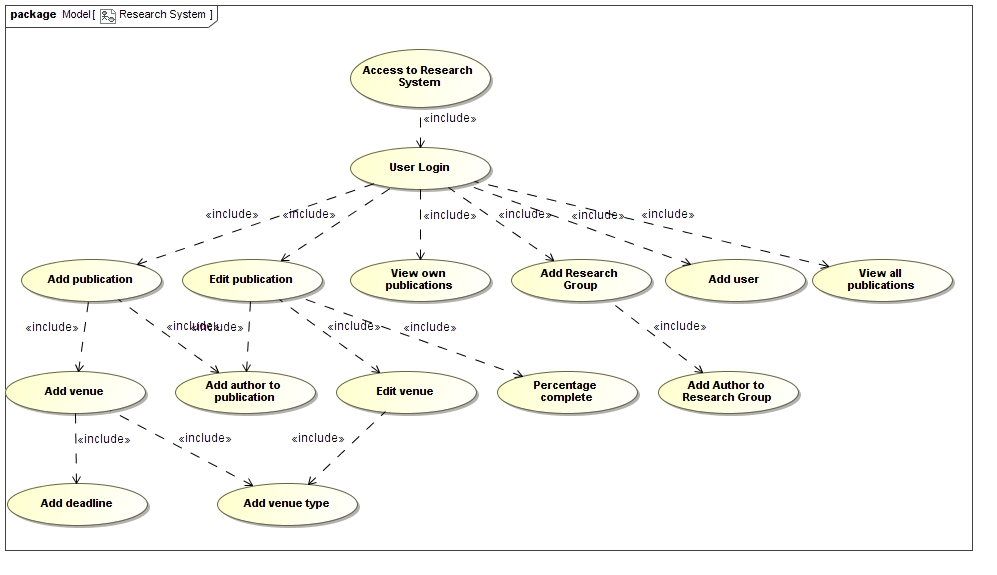
\includegraphics[width=\textwidth]{Overview.jpg}
		\caption{Functional Requirements: Overview of Research System \label{overflow}}
	\end{figure}
	\begin{figure}[H]
		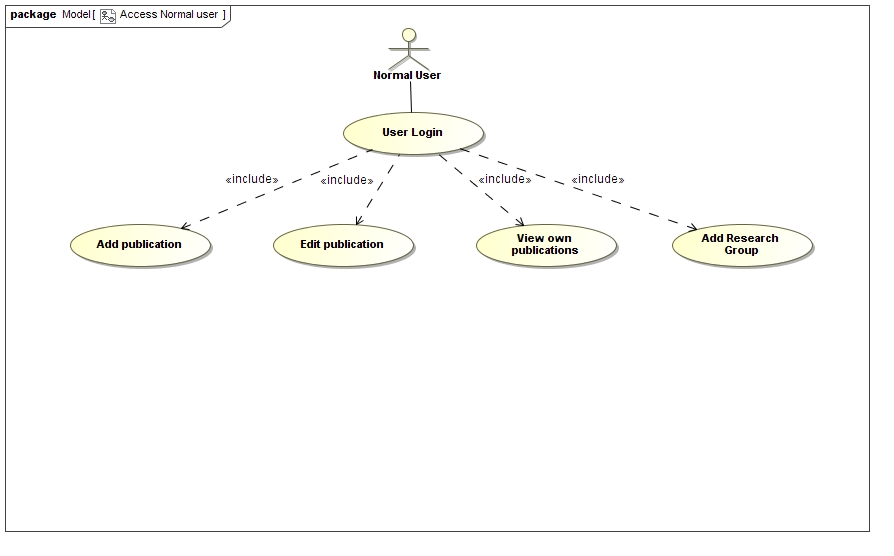
\includegraphics[width=\textwidth]{AccessNormaluser.jpg}
		\caption{Functional Requirements: Normal user access privileges \label{overflow}}
	\end{figure}
	\begin{figure}[H]
		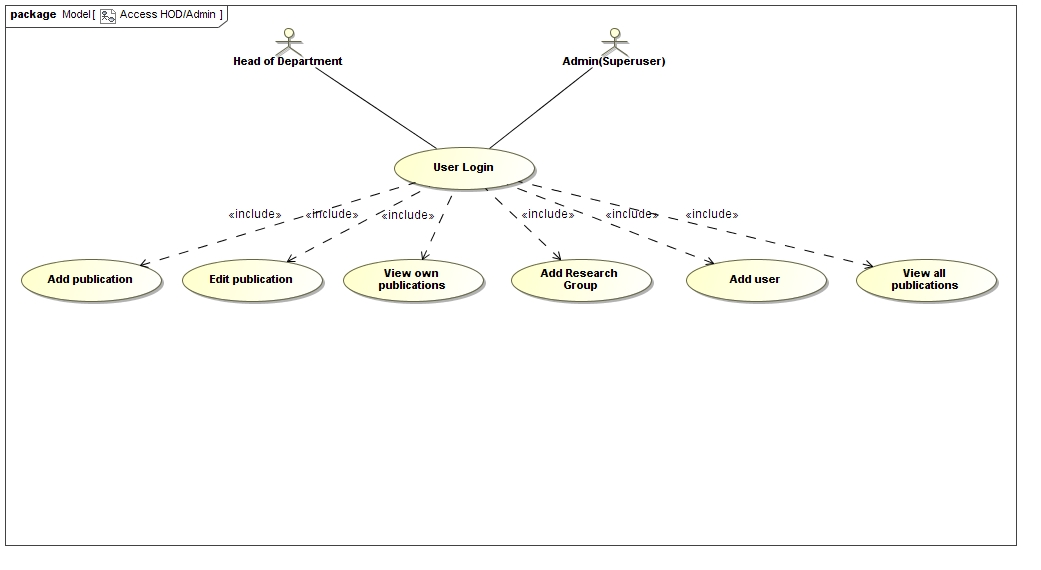
\includegraphics[width=\textwidth]{AccessHODAdmin.jpg}
		\caption{Functional Requirements: Superuser(HOD and admin) access privileges \label{overflow}}
	\end{figure}
	\subsection{Process Specification}
	\subsection{Domain Model}
	
	
	\section{Open Issues}
	
	
\end{document}
